\chapter{Results and Evaluation}\label{results-and-evaluation}

\section{Evaluation}\label{evaluation}

Before the results of the presented proof-of-concept implementation are listed it needs to be clear what dimensions are important so that a distinction between good and bad results can be made.

A good reprojection map has several qualities that make it usable as an obstacle gridmap. First, it needs to be \textbf{timely}. That means that the time between the appearance of an object in the robot's path and it being mapped in an obstacle map needs to be small enough that the robot can still avoid collisions. The \textbf{false alarm rate}, representing false positive detections, needs to be low enough to not negatively influence the robot's navigation behaviour by making it circumnavigate too many phantom obstacles. Vice versa, the \textbf{missed target rate}, or false negative detection needs to be low, or the radar sensor will not bring an advantage over conventional obstacle sensors. The resulting map of course also needs to be \textbf{spatially correct}. This means that a detected obstacle is mapped at its true location. Otherwise, phantom obstacles or incorrectly sized obstacles will degrade map quality. The map becomes more useful if it contains \textbf{diverse types of obstacles}, and not just one class of objects, like walls. On the other hand, it should not contain \textbf{irrelevant information}, for example wall humidity is not interesting for obstacle detection. Lastly, only if the map is \textbf{comparable to other sensors} informed comparison can take place. For example, a glass wall is easily visible to the human eye, so their position in the radar reprojection map can be verified. But metal struts in walls, which, while not presenting an obstacle to the robot (vacuum robots usually are not designed to breach walls), could be useful landmarks for later slam applications, are not visible in other maps. Hence the quality of metal strut mapping can not be asserted, but only assumed based on human knowledge of where a wall's metal struts might be.

There are some classes of targets that are particularly interesting in the evaluation of results. The first one is stacks of \textbf{metal cans}, because they appear in many of the scans. This is a kind of artificial obstacle that was designed to have a high probability of visibility in both radar scans (the curved metal surface is very reflective from every direction) and lidar scans (the can towers are high enough to cross the laser beam, and wide enough to not be missed even in some distance). Another easy target are \textbf{walls}. They are easy to see in the lidar scan, and detections in the radar reprojection map can be easily compared. A special case of walls are \textbf{glass walls} or windows. They present an impenetrable obstacle in a robots path, but almost always, neither a laser scanner nor a vision sensor can detect them (see \cref{fig:rgbd_glasswall2}). Another real world obstacle that escapes lidar scans are \textbf{office chair legs}. While the pillar is visible with laser, the horizontally stretching legs and rollers are usually too low to be detected (see \cref{fig:lidar_rgbd2}). In the same category of low profile obstacles are \textbf{cables} lying on the floor. A vacuum robot can easily entangle in them and get stuck. Lastly, it would be interesting to see negative obstacles including \textbf{cliffs} and dips. Today, robots need an extra set of sensors (usually IR distance sensors at the front of the robot, aiming at the floor) to detect this kind of obstacle very reliably.

\begin{figure}
    \begin{subfigure}[t]{.485\textwidth}
        \centering
        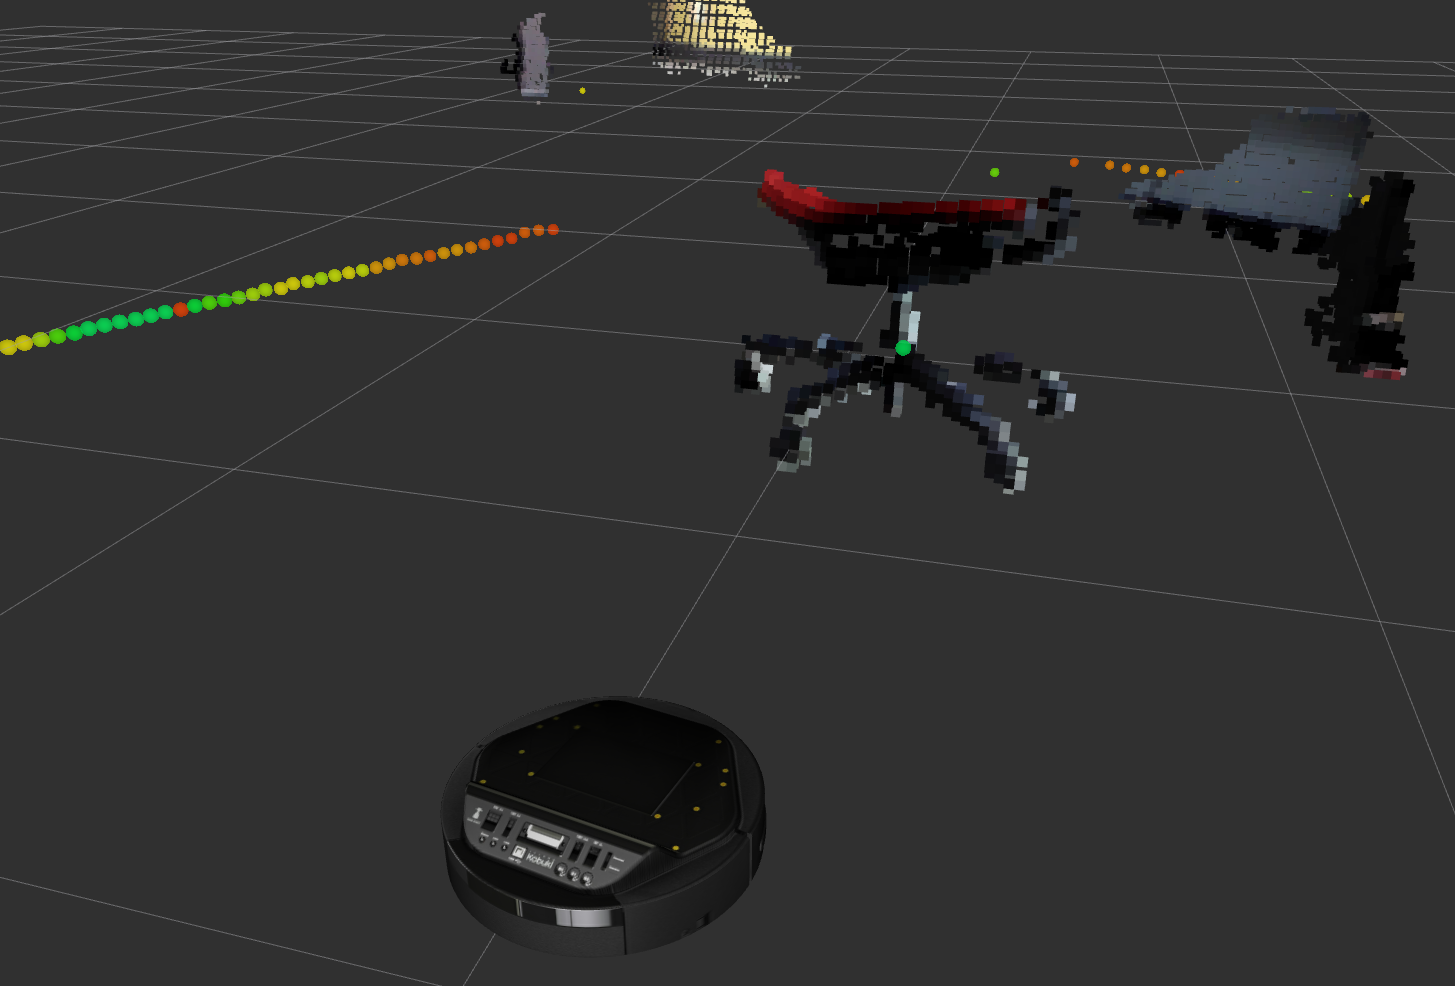
\includegraphics[max width=\textwidth]{gfx/screenshots/chair_laser_vs_rgbd}
        \caption{Laser fails to detect horizontal chair legs.}
        \label{fig:lidar_rgbd2}
    \end{subfigure}%
    \hfill%
    \begin{subfigure}[t]{.485\textwidth}
        \centering
        \def\svgwidth{\linewidth}
        \input{gfx/screenshots/rgbd_glasswall.pdf_tex}
        \caption{RGBD camera can not detect glass surface.}
        \label{fig:rgbd_glasswall2}
    \end{subfigure}%
    \caption{RViz screenshots showing traditional sensor shortcomings.}
\end{figure}


\section{Results}\label{results}

During development of the reprojection method, over 30 scans were taken. The environment for the scans is the BSH office in the Bosch Research and Technology Center in Palo Alto, which is fairly representative of a typical office environment. It has carpet floors, desks, office chairs, walls, corridors, and even glass walls.

The scans of this environment are assigned code names in alphabetical order for easy referencing. \Cref{tab:params} shows the parameters with which each of the scans was taken: Sweep time, sensor orientation (\textbf{H}orizontal / \textbf{V}ertical / \textbf{H}orizontal \textbf{I}nverted beam fan), squint angle (center of sensor's FOV, so \ang{90} is sideways-looking and \ang{0} is forward-looking), mounted horn antenna extension (which narrows the beam shape), availability of \texttt{/map} rosmessages with lidar slam information, and finally availability of \texttt{/tf} rosmessages which carry the slam-based odometry drift correction.

The scans are presented through the following plots:
\begin{itemize}
    \item Preprocessed (i.e. oversampled, range and transmit crosstalk compensated) input energy of range scans (down range echo intensity vs.~cross-range/mileage)
    \item Estimated Doppler speed, averaged over cross range as described in \cref{raw-data-smoothing} and peak FWHM as described in \cref{peaks-overlaps-at-crossing-target-arcs}
    \item DOA estimation (described in \cref{doa-implementation}) to resolve the angle ambiguities described in \cref{geometry-for-the-general-case}. Likewise averaged over cross-range and FWHM.
    \item Reprojection map as described in \cref{reprojection-mapping}
    \item If the \texttt{/map} is available for a scan, also the overlay of reprojection map and lidar occupancy gridmap as described in \cref{output}.
\end{itemize}

\begin{table}[htb]
    \rowcolors{1}{ColorAlternatedRow}{}
    \begin{tabularx}{\textwidth}{%
      >{\setlength{\hsize}{.31\hsize}\raggedright\arraybackslash}X%
      >{\setlength{\hsize}{.15\hsize}\raggedright\arraybackslash}X%
      >{\setlength{\hsize}{.12\hsize}\raggedright\arraybackslash}X%
      >{\setlength{\hsize}{.12\hsize}\raggedright\arraybackslash}X%
      >{\setlength{\hsize}{.10\hsize}\centering\arraybackslash}X%
      >{\setlength{\hsize}{.10\hsize}\centering\arraybackslash}X%
      >{\setlength{\hsize}{.10\hsize}\centering\arraybackslash}X%
    }
    \hiderowcolors
    \toprule
Name & Sweep & Orient. & Squint & Horn & Map & TF \\
    \midrule
    \endhead
    
    \bottomrule
    \endfoot
    \showrowcolors
    %
 Attic & \SI{5.0}{ms} & H & \ang{90} & \cmark & \xmark & \xmark \\
 Basement & \SI{5.0}{ms} & H & \ang{90} & \cmark & \xmark & \xmark \\
 Cafeteria & \SI{5.0}{ms} & H & \ang{90} & \cmark & \xmark & \xmark \\
 Dungeon & \SI{5.0}{ms} & V & \ang{20} & \cmark & \xmark & \xmark \\
 Entryway & \SI{5.0}{ms} & V & \ang{20} & \cmark & \xmark & \xmark \\
 Fallout shelter & \SI{5.0}{ms} & V & \ang{20} & \cmark & \xmark & \xmark \\
 Garden & \SI{5.0}{ms} & V & \ang{20} & \cmark & \xmark & \xmark \\
 Home cinema & \SI{5.0}{ms} & V & \ang{20} & \cmark & \xmark & \xmark \\
 Indoor swimming pool & \SI{5.0}{ms} & V & \ang{20} & \cmark & \xmark & \xmark \\
 Jail cell & \SI{5.0}{ms} & H & \ang{20} & \cmark & \xmark & \xmark \\
 Kitchen & \SI{5.0}{ms} & H & \ang{20} & \xmark & \xmark & \xmark \\
 Lobby & \SI{5.0}{ms} & H/I & \ang{0} & \xmark & \xmark & \xmark \\
 Mancave & \SI{5.0}{ms} & H/I & \ang{0} & \xmark & \xmark & \xmark \\
 Nirvana & \SI{5.0}{ms} & H/I & \ang{0} & \xmark & \cmark & \xmark \\
 Orbit & \SI{5.0}{ms} & H/I & \ang{0} & \xmark & \cmark & \xmark \\
 Public Restroom & \SI{5.0}{ms} & H/I & \ang{0} & \xmark & \cmark & \cmark \\
 Queue & \SI{20}{ms} & H/I & \ang{0} & \xmark & \cmark & \cmark \\
 Racetrack & \SI{2.0}{ms} & H/I & \ang{0} & \xmark & \cmark & \cmark \\
 Sauna & \SI{2.5}{ms} & H/I & \ang{0} & \xmark & \cmark & \cmark \\
 Torture Chamber & \SI{2.5}{ms} & H/I & \ang{45} & \xmark & \cmark & \cmark \\
 Underground & \SI{2.5}{ms} & H/I & \ang{45} & \xmark & \cmark & \cmark \\
 Virtual Reality & \SI{2.5}{ms} & H/I & \ang{45} & \xmark & \cmark & \cmark \\
 Washroom & \SI{2.5}{ms} & V & \ang{45} & \xmark & \cmark & \cmark \\
 Xray-Room & \SI{2.5}{ms} & V & \ang{0} & \xmark & \cmark & \cmark \\
 Y is there a cable on the floor & \SI{5.0}{ms} & V & \ang{0} & \xmark & \cmark & \cmark \\
 Z & & & & & & \\
    \end{tabularx}
    \caption{Scan parameters}
    \label{tab:params}
\end{table}


An exemplary result is shown in \cref{fig:nirvana}. More result plots can be found in \cref{scans}

\begin{figure}[htbp]
    \centering
    \begin{subfigure}[t]{0.32\linewidth}
        \centering
        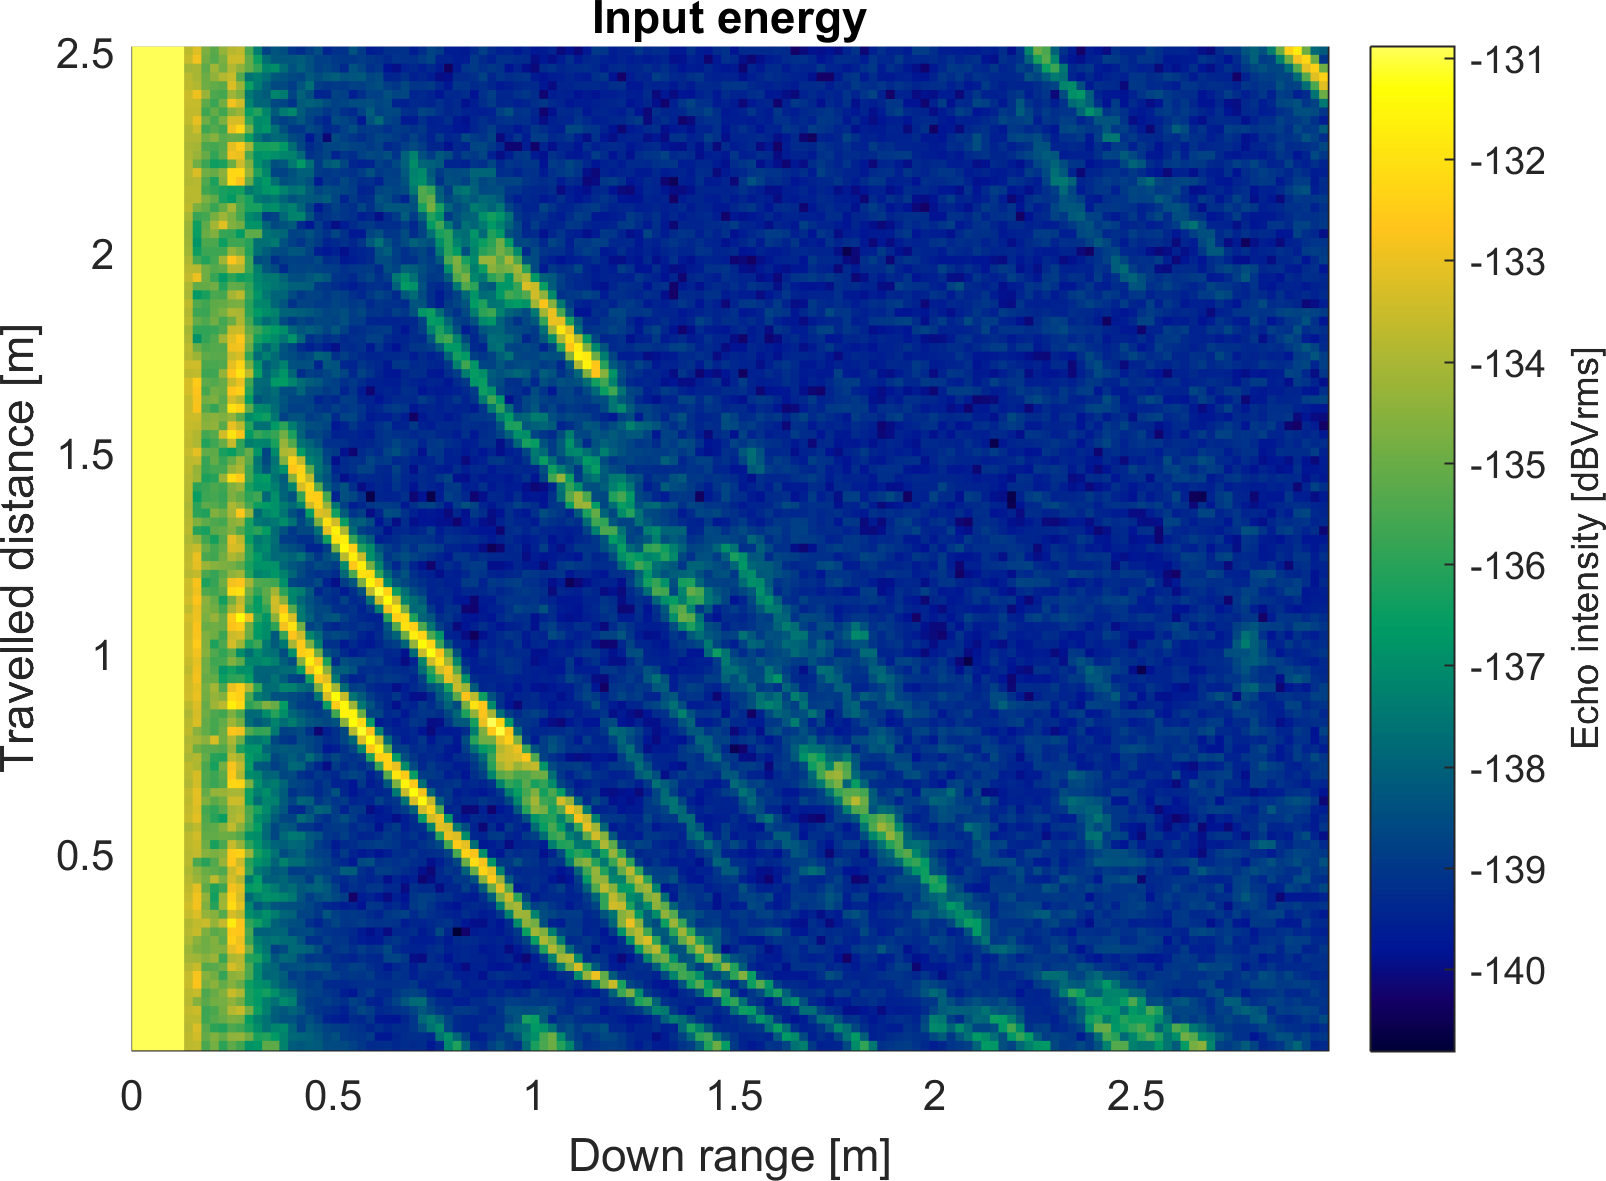
\includegraphics[width=\linewidth]{gfx/results/nirvana_input.png}
        \caption{\small Input energy}
    \end{subfigure}%
    \hfill%
    \begin{subfigure}[t]{0.32\linewidth}  
        \centering 
        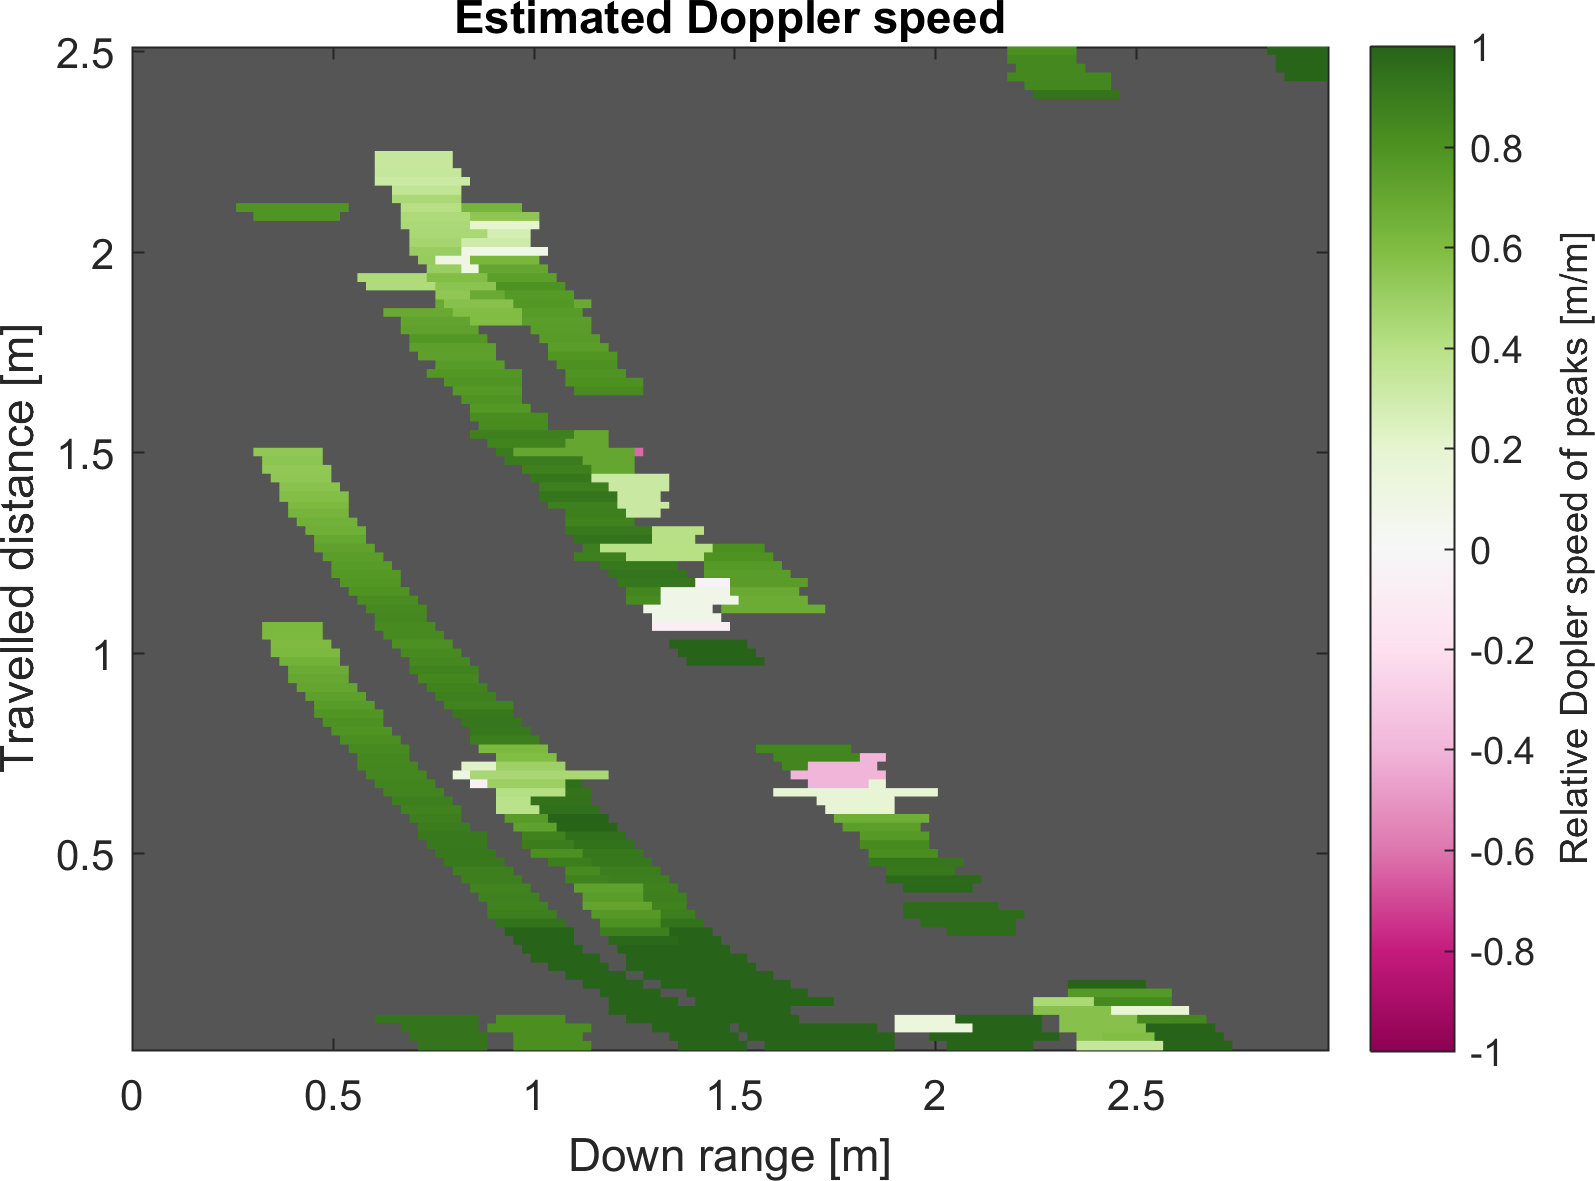
\includegraphics[width=\linewidth]{gfx/results/nirvana_doppler.png}
        \caption{\small Doppler estimation}
    \end{subfigure}%
    \hfill%
    \begin{subfigure}[t]{0.32\linewidth}   
        \centering 
        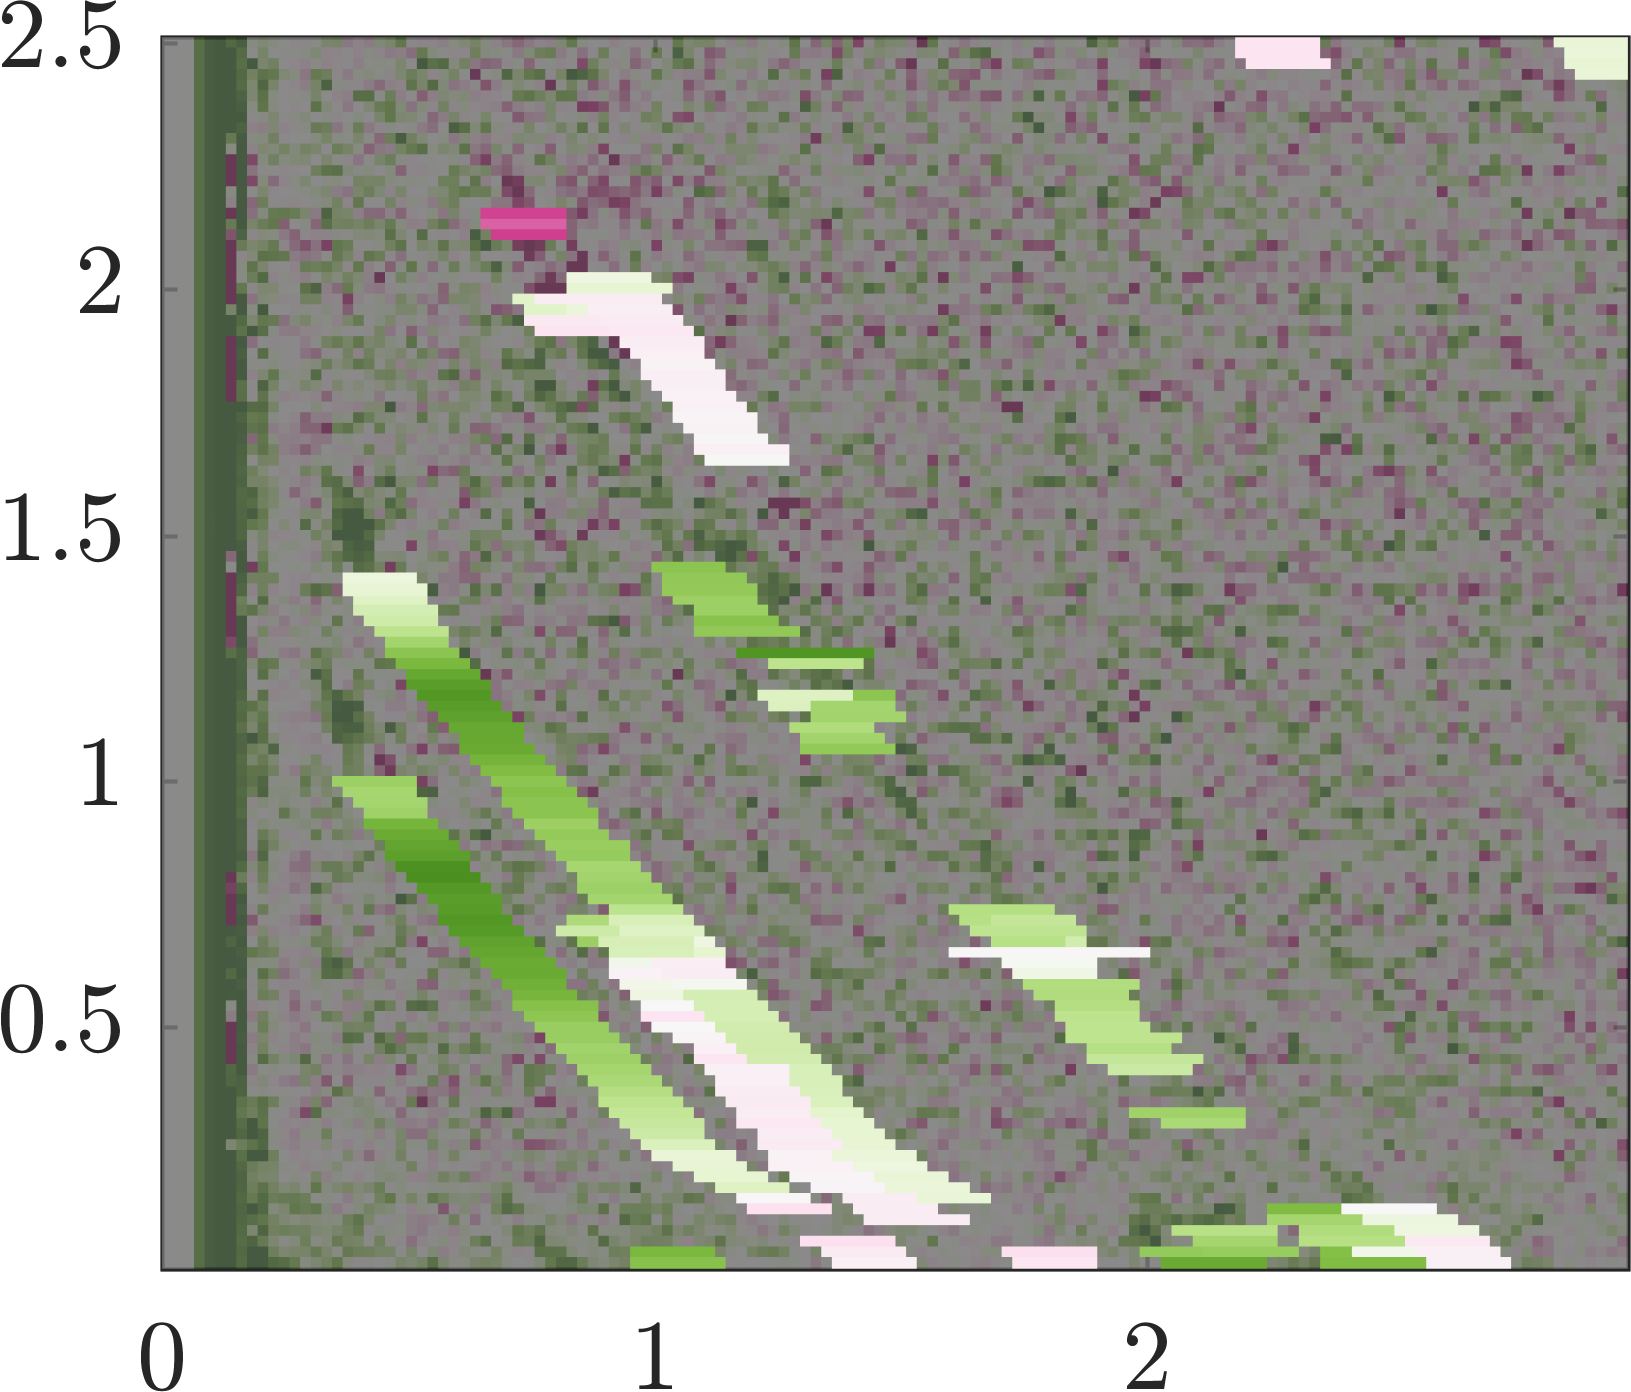
\includegraphics[width=\linewidth]{gfx/results/nirvana_doa.png}
        \caption{\small Direction of Arrival}
    \end{subfigure}\\
    \begin{subfigure}[t]{0.475\textwidth}   
        \centering 
        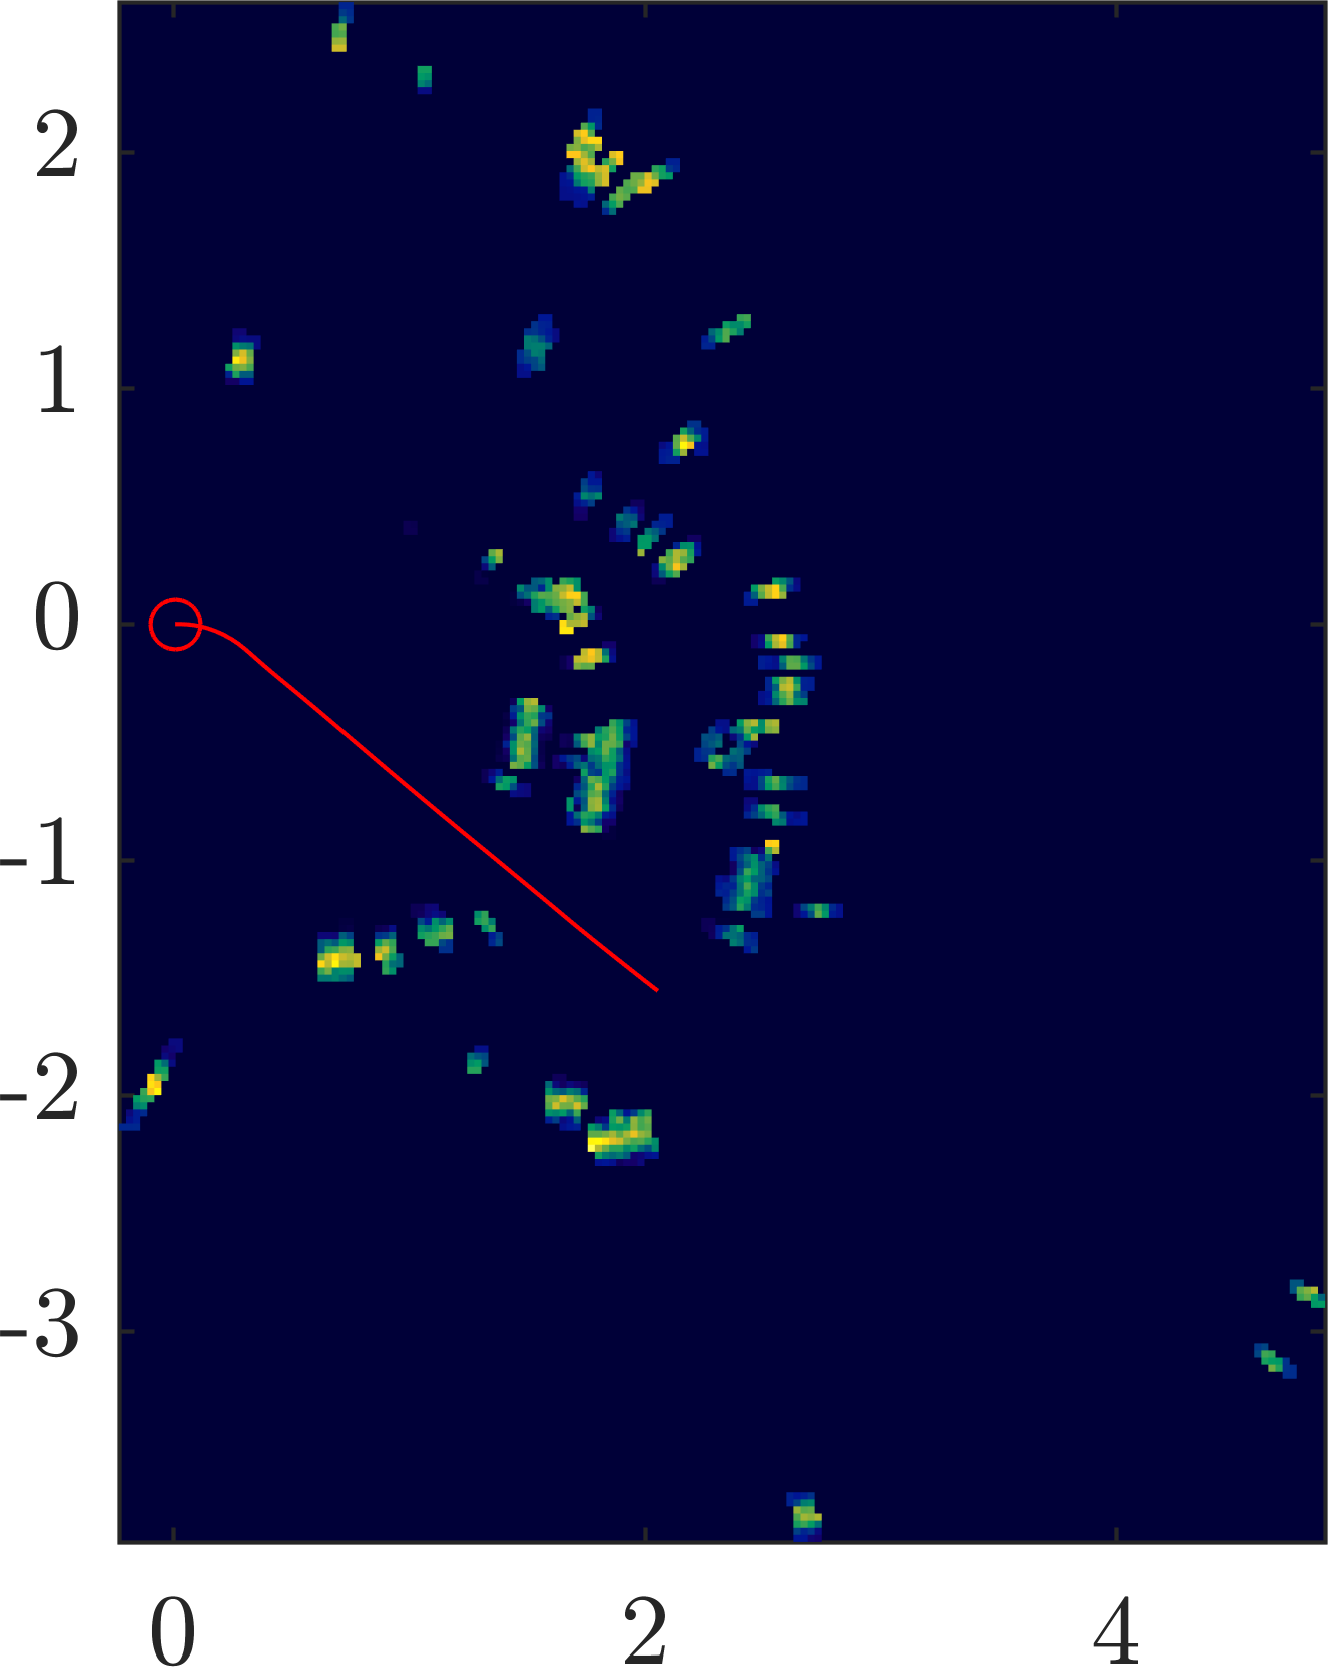
\includegraphics[max width=\linewidth, max height=\linewidth]{gfx/results/nirvana_reprojection.png}
        \caption{\small Reprojection Map}
    \end{subfigure}%
    \hfill%
    \begin{subfigure}[t]{0.475\textwidth}   
        \centering 
        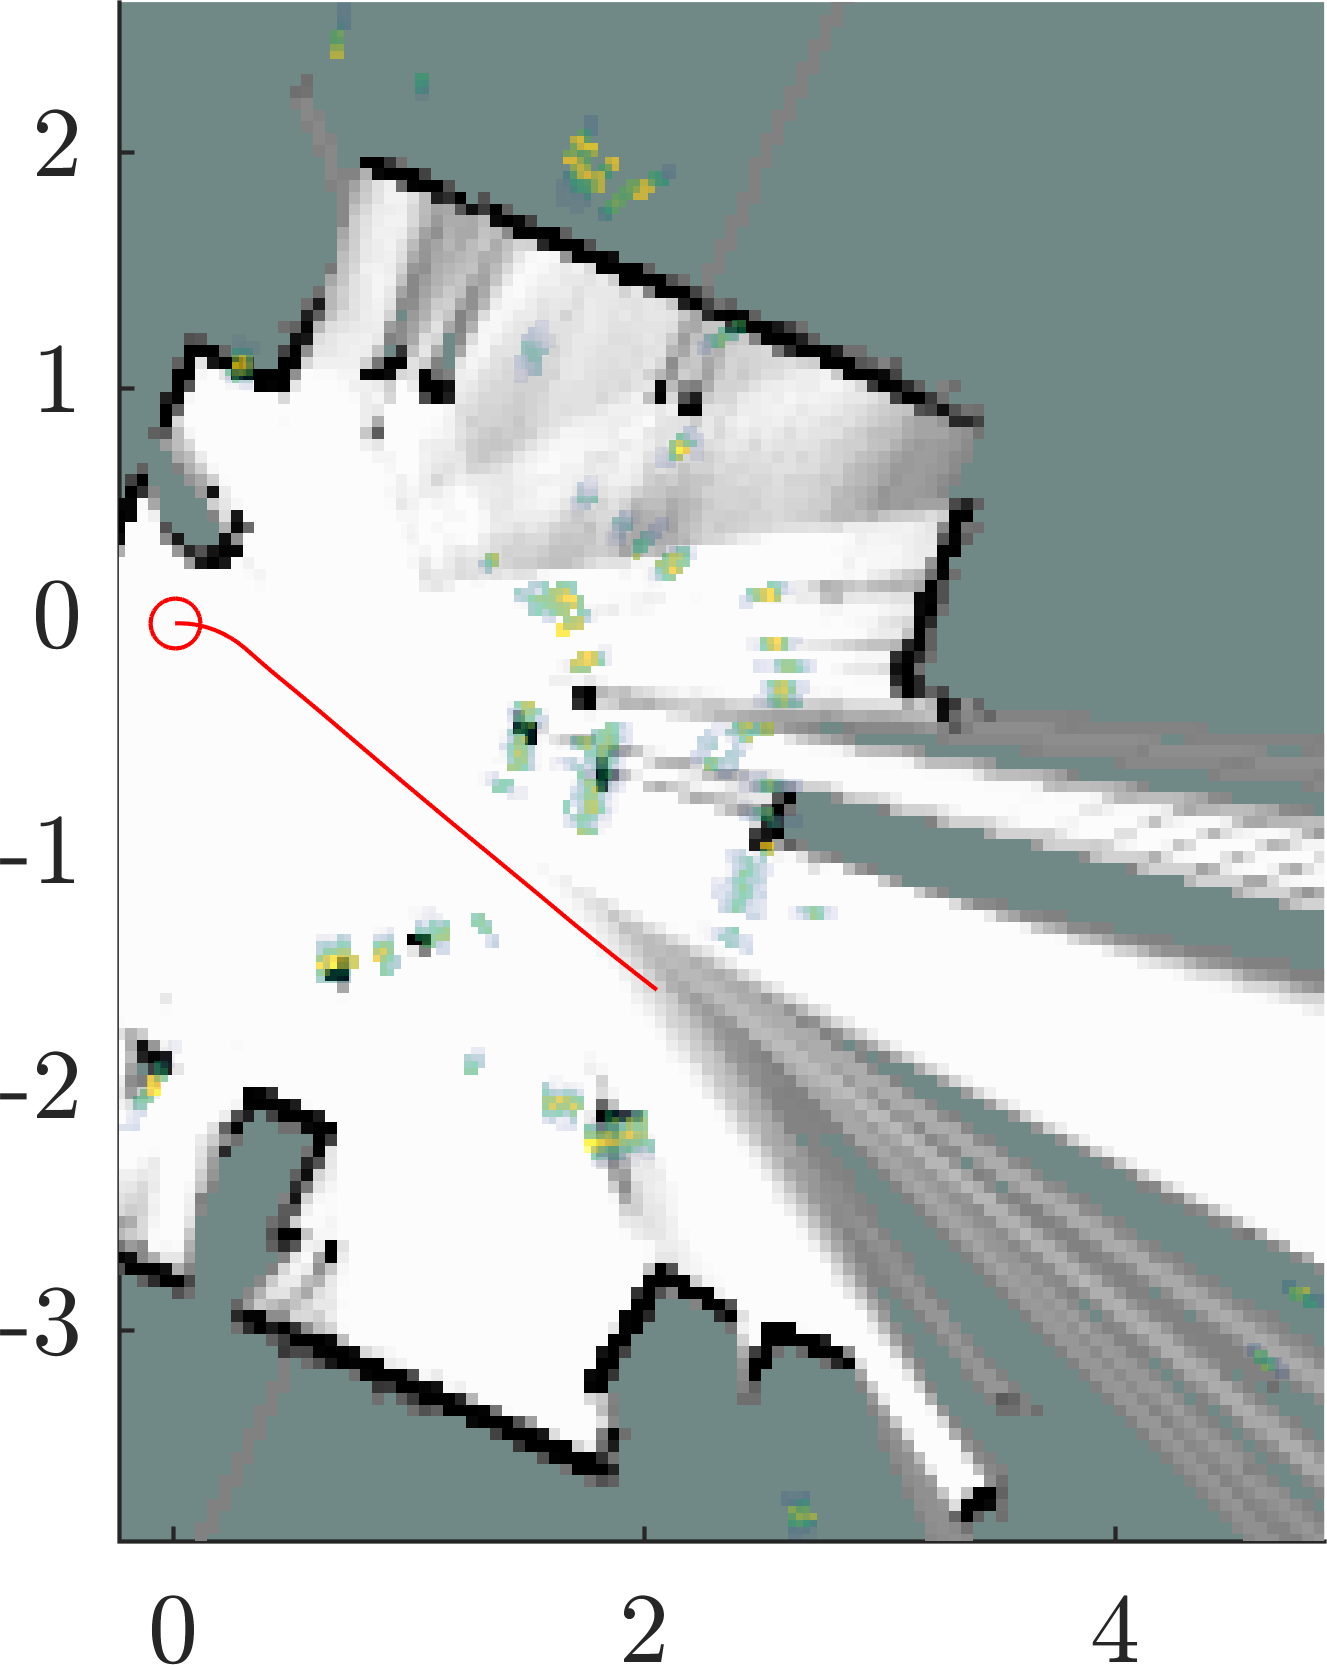
\includegraphics[max width=\linewidth, max height=\linewidth]{gfx/results/nirvana_map.png}
        \caption{\small Reprojection Map}
    \end{subfigure}%
    \caption{Nirvana scan} \label{fig:nirvana}
\end{figure}

